\renewcommand{\chaptername}{Cap\'itulo}
\chapter{Planteamiento del problema} 

\section{Introducci\'on al acceso abierto}

El acceso abierto (AA, del ing\'es \emph{Open Access}) a la literatura es digital, en l\'inea, libre de cargo y libre de la mayor\'ia de restricciones de derechos de autor y licencias; elimina las barreras de precios por suscripciones, cuotas o pago de licencias \cite{PeterSuber2015}.\newline

%% DANIEL, ENTRA A ESTE ENLACE Y CONSTRUYE UNA ENTRADA EN BIBTEX PARA ESTE ENLACE: http://legacy.earlham.edu/~peters/fos/overview.htm
%% YA QUEDO

Existen diversos tratados y convenciones internacionales que promueven el AA del p\'ublico en general a la literatura cient\'ifica y acad\'emica de manera digital representada en revistas cient\'ificas, de divulgaci\'on, tesis, art\'iculos, memorias de eventos, libros, entre otros recursos. La propuesta del AA se plante\'o en la Iniciativa de Budapest en 2002, durante un evento organizado por el \textit{Open Society Institute}, (Instituto de la Sociedad Abierta); en 2003, se llev\'o a cabo la Declaraci\'on de Berl\'in sobre el AA al conocimiento en las ciencias y las humanidades \cite{para2010abierto}.

Para \cite{BeneficiosAA}, el AA ofrece a las Instituciones de Edu\-caci\'on Superior (IES) y Centros de Investigaci\'on (CIs) beneficios como los siguientes: 
\begin{itemize}
\item Rendici\'on de cuentas transparente ante la sociedad con respecto a la inversi\'on p\'ublica
\item Incremento en la difusi\'on e impacto de la producci\'on cient\'ifica  
\item Fomento de la producci\'on cient\'ifica y acad\'emica incrementando las posibilidades de acceso 
\item Dis\-mi\-nu\-ci\'on en la brecha de acceso a la informaci\'on entre IES, CIs, comunidades locales, nacionales e internacionales
\item Garantiza la preservaci\'on electr\'onica de los recursos documentales
\end{itemize}
 
Entre los beneficiarios del AA est\'an los autores, las comunidades cient\'ificas y acad\'emicas, as\'i como los usuarios finales. El AA se relaciona con el uso, desarrollo e implementaci\'on de \emph{repositorios institucionales}, que son plataformas tecnol\'ogicas dise\~{n}adas para almacer, preservar y difundir documentos digitales que se distribuyen bajo los t\'erminos de las pol\'iticas de AA, su prop\'osito es ser un medio de divulgaci\'on (\textit{ruta verde}) o de publicaci\'on (\textit{ruta dorada}), de los contenidos producidos por una instituci\'on o comunidad \cite{RutaVerdeDorada}.
%% DANIEL, AGREGA UNA CITA PARA LO DE LA RUTA VERDE Y DORADA
%% YA QUEDO
\subsection{Panorama general de los repositorios digitales}

%% DANIEL, AGREGA LA DEFINICION DE UN REPOSITORIO INSTITUCIONAL QUE PROVENGA DE UN LIBRO AQUI
%% YA QUEDO

Según \cite{EcosistemasdelAA}, un repositorio institucional es un conjunto de servicios prestados por las universidades y organismos de investigación, al conjunto de la comunidad, para recopilar, administrar, difundir, y preservar la producción documental digital generada en la Institución, cualquiera que sea su tipología, a través de la creación de una colección digital organizada, abierta e interoperable a través del protocolo OAI-PMH, con el fin de garantizar un aumento en la visibilidad e impacto de la misma.\newline

En Diciembre de 2018, seg\'un el sitio OpenDOAR \cite{OpenDOAR}, directorio de repositorios de AA de la Universidad Nottingham, exist\'ian tres mil setecientos setenta y nueve repositorios de AA alrededor del mundo, de los cuales (46\%) se encuentran en Europa (46\%), el 27\% en Norteam\'erica y s\'olo el 0.9\% en M\'exico. En Septiembre del 2019, la p\'agina web del Repositorio Nacional (RN) \cite{RepositorioNacional} reporta la existencia de 100 repositorios de Ciencia Abierta (CA) e INDEXE, Sistema de B\'usqueda de la Red Mexicana de Repositorios Institucionales (REMERI) \cite{RI_REMERI} indica tambi\'en 100 repositorios institucionales (RIs) comprometidos con la divulgaci\'on de sus contenidos institucionales y tem\'aticos bajo las pol\'iticas de AA.\newline

De acuerdo con el \textit{software} empleado para la implementaci\'on de repositorios digitales (RDs), OpenDOAR \cite{OpenDOAR} se\~{n}ala que las cuatro plataformas m\'as empleadas a nivel mundial son: \textit{DSpace} \cite{DSpaceRef} (44.2\%), \textit{EPrints} (13.4\%), \textit{Digital Commons} (4.7\%) y \textit{WEKO} (2.7\%). A diferencia de \textit{Digital Commons} que es un \textit{software} licenciado por la empresa \textit{Beprees}, \textit{WEKO}, \textit{EPrints} y \textit{DSpace} cuentan con licencia libre, por lo que su uso se ha extendido en m\'ultiples IES, CIs y otras organizaciones.\newline

\textit{EPrints} \cite{EPrints} es un software de uso libre desarrollado en el a\~{n}o 2000 por la Universidad de Southampton en el Reino Unido, esta plataforma soporta la preservaci\'on, diseminaci\'on y generaci\'on de reportes para instituciones que requieran que servicios de AA, tambi\'en permite el desarrollo de repositorios de educaci\'on abierta (en ingl\'es \textit{Open Education}) y bancos de datos para investigaci\'on (en ingl\'es \textit{Research Data}). EPrints ofrece integraci\'on con redes sociales, por lo que se emplea como medio de integraci\'on entre comunidades estudiantiles y acad\'emicas.\newline

\textit{DSpace} \cite{DSpaceRef} surgi\'o com proyecto desarrollado en sus inicios por el Instituto Tecnol\'ogico de Massachusetts (MIT) en el a\~{n}o 2002 en conjunto con los Laboratorios HP. Actualmente, se mantiene en la fundaci\'on \textit{DuraSpace} que entre sus objetivos se encuentran la innovaci\'on en tecnolog\'ias de AA y basadas en nube, principalmente para bibliotecas, universidades, CIs y organizaciones de patrimonio cultural. DSpace soporta el almacenamiento de tesis, administraci\'on de registros electr\'onicos, preservaci\'on digital y publicaci\'on. Los RIs que interoperan con el RN \cite{RepositorioNacional} emplean en su mayor\'ia (m\'as del 90\%) una versi\'on de DSpace.  Una comparaci\'on que considera aspectos de funcionalidad, elementos t\'ecnicos y de administraci\'on entre DSpace e EPrints se presenta en \cite{EvaluacionDeUsabilidad}.\newline

A diferencia de EPprints y DSpace en las que la interoperabilidad en la configuraci\'on por omisi\'on se implementa al utilizar el protocolo  OAI-PMH\footnote{Open Archives Initiative Protocol for Metadata Harvesting} \cite{Lagoze2005} y el est\'andar de metadatos Dublin Core \cite{DublinCore}, existen otras alternativas de software para la implementaci\'on de RDs que gestionan informaci\'on sem\'antica tales como VIVO \cite{VivoWeb}, que es una plataforma de AA desarrollada por la Universidad de Cornell, en el a\~{n}o 2003, \'esta incluye un m\'odulo de modelos sem\'anticos u ontolog\'ias como \textit{Dublin Core} \footnote{Disponible en http://dublincore.org/} , \textit{Bibliographic Ontology} \footnote{Disponible en http://bibliontology.com/}, \textit{FOAF} \footnote{Disponible en http://www.foaf-project.org/} y \textit{SKOS} \footnote{Disponible en http://www.w3.org/2004/02/skos/}. 
Otra plataforma que emplea tecnolog\'ias sem\'anticas es \emph{Virtuoso}, \'esta se desarroll\'o en Espa\~{n}a por la empresa OpenLink\cite{VirtuosoRef}; algunas de sus aplicaciones son servicios web, bases de datos, web sem\'antica, sistemas inteligentes, exportaci\'on e importaci\'on de documentos en m\'ultiples formatos, documentos compartidos a trav\'es de la nube, \emph{blogs}, \emph{wikis}, correo personalizado y modelos de negocios.\newline

El RI de la Universidad Polit\'ecnica de Puebla, en adelante RI-UPPue, est\'a implementado en DSpace. En esta tesis se identifica como problem\'atica para la comunidad universitaria lo siguiente:

\begin{itemize}
\item Los mecanismos de recuperaci\'on de informaci\'on disponibles desde la interfaz del RI-UPPue s\'olo distinguen entre el autor principal y los co-autores de los documentos; a la fecha, no se puede determinar un rol de los autores en el proceso de elaboraci\'on de los documentos como estudiante, asesor o sinodal si se trata de una tesis, o autor principal y co-autores si es un art\'iculo

\item Existe \textit{ambig\"{u}edad} en la interpretaci\'on de los datos descriptivos (o \emph{metadatos}) cuando se sube un documento al repositorio, por ejemplo, qu\'e se debe colocar dentro del elemento \emph{contributor} de una tesis de maestr\'ia

\item A pesar de que otras IES que interoperan con el RN comparten la misma plataforma, es decir, DSpace, la exportaci\'on de datos est\'a sujeta a la interpretaci\'on de los usuarios finales, dado que \'esta se realiza por omisi\'on \'unicamente en el formato CSV\footnote{CSV corresponde a las siglas de \emph{Comma Separated Values}}

\item La consulta de datos en m\'as de un repositorio que interopera con el RN se realiza a trav\'es de su propio sistema de b\'usqueda, esto implica que los usuarios est\'an limitados a encontrar los documentos de inter\'es s\'olo por algunos metadatos y no los 15 que forman parte del est\'andar Dublin Core \cite{DublinCore}

\end{itemize}

Finalmente, la ontolog\'ia Onto4AIR es un modelo formal legible por una computadora que, reduce la ambiguedad y representa el dominio y operaci\'on del conocimiento de un repositorio institucional \cite{representacionSemantica}.

Dada la problem\'atica anterior, esta tesis propone los objetivos siguientes. 

\section{Objetivo general} 

Implementar un servicio web tipo REST dise\~{n}ado para extender los mecanismos de b\'usqueda de tesis, art\'iculos y carteles del RI-UPPue utilizando tecnolog\'ias sem\'anticas 

\subsection{Objetivos espec\'ificos}

\begin{itemize}
     \item  Integrar datos de tesis de maestr\'ia, art\'iculos y carteles del RI-UPPue a la ontolog\'ia Onto4AIR como instancias validando su consistencia l\'ogica de forma autom\'atica mediante razonadores

     \item Describir la funcionalidad del componente RDF de la plataforma DSpace 6.2, Virtuoso y Vivo relacionada con la representaci\'on y recuperaci\'on de informaci\'on sem\'antica
     
     \item Dise\~{n}ar e implementar un servicio web que permita recuperar datos de dos RIs que interoperen con el RN utilizando tecnolog\'ias sem\'anticas
   \end{itemize}
   
   
La Figura \ref{actividades_objetivos} muestra algunas de las tareas requeridas para alcanzar los objetivos de esta tesis. 

\begin{figure}[!ht]
    \centering
    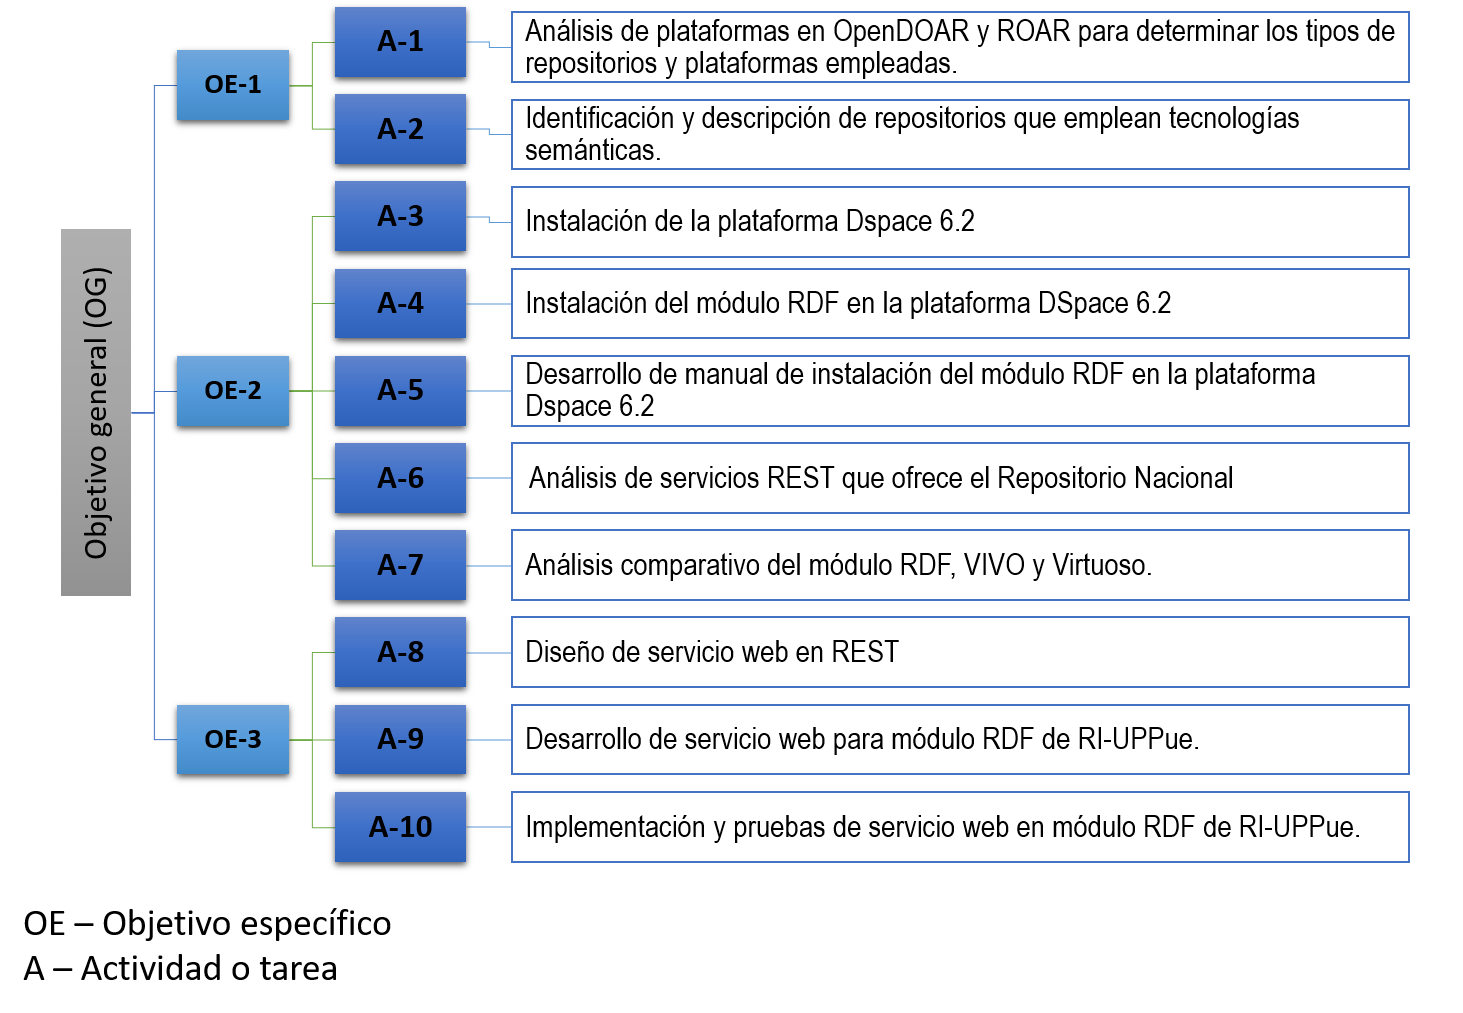
\includegraphics[width=12cm]{figures/Actividades_Dic_2018.png} %NOMBRE DE LA FIGURA y TAMANIO
    \caption{Tareas a desempe\~{n}ar para el desarrollo del servicio web} %PIE DE LA IMAGEN
    \label{actividades_objetivos}
\end{figure}

\section{Justificaci\'on}

En los \'ultimos a\~{n}os, diferentes IES, CIs y comunidades se han sumado el esfuerzo de promover el AA a sus contenidos cient\'ificos, aprovechando al mismo tiempo los beneficios generados por la implantaci\'on de un RD. Entre las ventajas que representa el uso de las ontolog\'ias y los modelos de datos no relacionales se mencionan las siguientes: \cite{ASWebQuest} \cite{GuideCreatingOntology}

\begin{itemize}
\item \textit{Intercambio de informaci\'on} entre aplicaciones, programas y/o plataformas trav\'es del uso del lenguaje XML.
\item \textit{Datos incompletos}, es decir, a pesar de que algunos datos no est\'en contenidos en la base, a\'un as\'i la ontolog\'ia puede arrojar resultados a las consultas formuladas por los usuarios.
\item \textit Las ontolog\'ias permiten el manejo de mayor {tipos de datos} que en una base de tipo relacional, lo cual permite realizar consultas espec\'ificas.
\item \textit Permiten la {reutilizaci\'on del conocimiento}, es decir, al recopilar la informaci\'on, \'esta se encuentra a disposici\'on de los usuarios para consultar o acrecentar la informaci\'on existente.
\item \textit{Analizar el dominio }del conocimiento, fijando l\'imites entre \'este y el conocimiento operacional.
\end{itemize}

En M\'exico, m\'as del 45\% de RI's pertenecen a instituciones p\'ublicas \cite{RI_REMERI}, siendo la Universidad Nacional Aut\'onoma de M\'exico - \textit{UNAM} la instituci\'on con mayor n\'umero de repositorios y documentos publicados. En este sentido, la Universidad Polit\'ecnica de Puebla actualmente participa en un proyecto que implementa un Repositorio Institucional (\textit{RI-UPPuebla}) en el cual sus investigadores, alumnos de posgrado y comunidad universitaria en general, difundir\'a y preservar\'a contenidos de car\'acter cient\'ifico y acad\'emico en AA, donde los beneficios esperados por tipo de usuario ser\'an:

- A los investigadores: 
	\begin{itemize}
	\item \textit{Publicaci\'on de los resultados} de su investigaci\'on al interior y exterior de la comunidad universitaria.
    \item \textit{Mayor n\'umero de citas}, al ser m\'as accesible al p\'ublico, causando mayor impacto.
    \item \textit{Gesti\'on} de los derechos de autor.
    \item \textit{Acceso permanente} a las publicaciones ya que los accesos no se modifican, como suele ocurrir en otros medios digitales.
    \item \textit{Almacenamiento flexible}, al permitir almacenar cualquier tipo de documentos como art\'iculos, tesis, revistas, memorias, videos, audios, etc. en formatos digitales.
	\end{itemize}
	
- A la UPPue:
	\begin{itemize}
	\item \textit{Recopilaci\'on y divulgaci\'on} la producci\'on cient\'ifica y acad\'emica de la instituci\'on.
    \item \textit{Visibilidad e impacto}, ya que al colocar mayor n\'umero de publicaciones en las b\'usquedas de diversos motores, posicionar\'a a la UPPue como referente en citas de docentes y estudiantes.
    \item \textit{Banco de conocimientos hacia el futuro}, al preservar las obras, el acervo do\-cu\-mental y de conocimientos crecer\'a con el paso del tiempo, lo cual fomentar\'a mayor actividad de investigaci\'on entre la comunidad universitaria, al contar con las bases cient\'ificas realizadas por sus pares e incluso sus predecesores.
	\end{itemize}
	
- A la comunidad universitaria:
  \begin{itemize}
  \item \textit{Acceso libre y gratuito} a obras cient\'ificas y acad\'emicas serias y de origen confiable.
  \item \textit{Cooperaci\'on y acceso} compartido entre las IES que conforman comunidades de conocimiento de la regi\'on, del pa\'is o de la comunidad internacional.
  \item \textit{Evidencias} tangibles de los resultados generados a trav\'es de la inversi\'on p\'ublica o privada de recursos en el campo de la investigaci\'on cient\'ifica o acad\'emica.
  \end{itemize}

Como parte del proceso de consolidaci\'on del RI-UPPue, se ha identificado como \'area de oportunidad explorar la informaci\'on almacenada y enriquecerla con otros datos que permitan encontrar informaci\'on impl\'icita. Si bien la mayor\'ia de las IES, CIs u otro tipo de organizaciones implementan herra\-mi\-en\-tas para la concentraci\'on y administraci\'on de informaci\'on en bases de datos, se requiere de las tecnolog\'ias sem\'anticas como medios para transformar los datos en conocimiento, lo cual permite acceder a la informaci\'on desde un punto de vista conceptual y no textual.

En suma, el desarrollo e implantaci\'on de un servicio de consultas sem\'anticas permit\'a extender los mecanismos de b\'usqueda y recuperaci\'on relacionada con los documentos y sus productores; en comparaci\'on con los mecanismos provistos actualmente en el RI-UPPue.


